\section{{\sys}}
%The objective of {\sys} is to efficiently manage inter-domain outbound traffic, switching it from the current {\egresses} to the newly planned ones. This aims to improve clients' access experiences and reduce inter-domain bandwidth costs. Figure \ref{fig:systemar} shows the infrastructure involved, which provides diverse information about flows from the WAN to {\sys} and steers the traffic to the specific egresses designated by the controller. {\sys} adopt a multi-phase optimization approach in \S\ref{sec:te} to address the challenges of scheduling in the presence of limited backbone links. Given the considerable scale of optimization involved, we employ several techniques in \S\ref{sec:overall-slu} and \S\ref{sec:timeslot-slu}  to make the problem solvable, first from being unsolvable to being solvable but time-consuming, and then from being solvable but time-consuming to being solvable very quickly, which meets the deployment requirements.

\iffalse
\begin{figure}
	\centering
	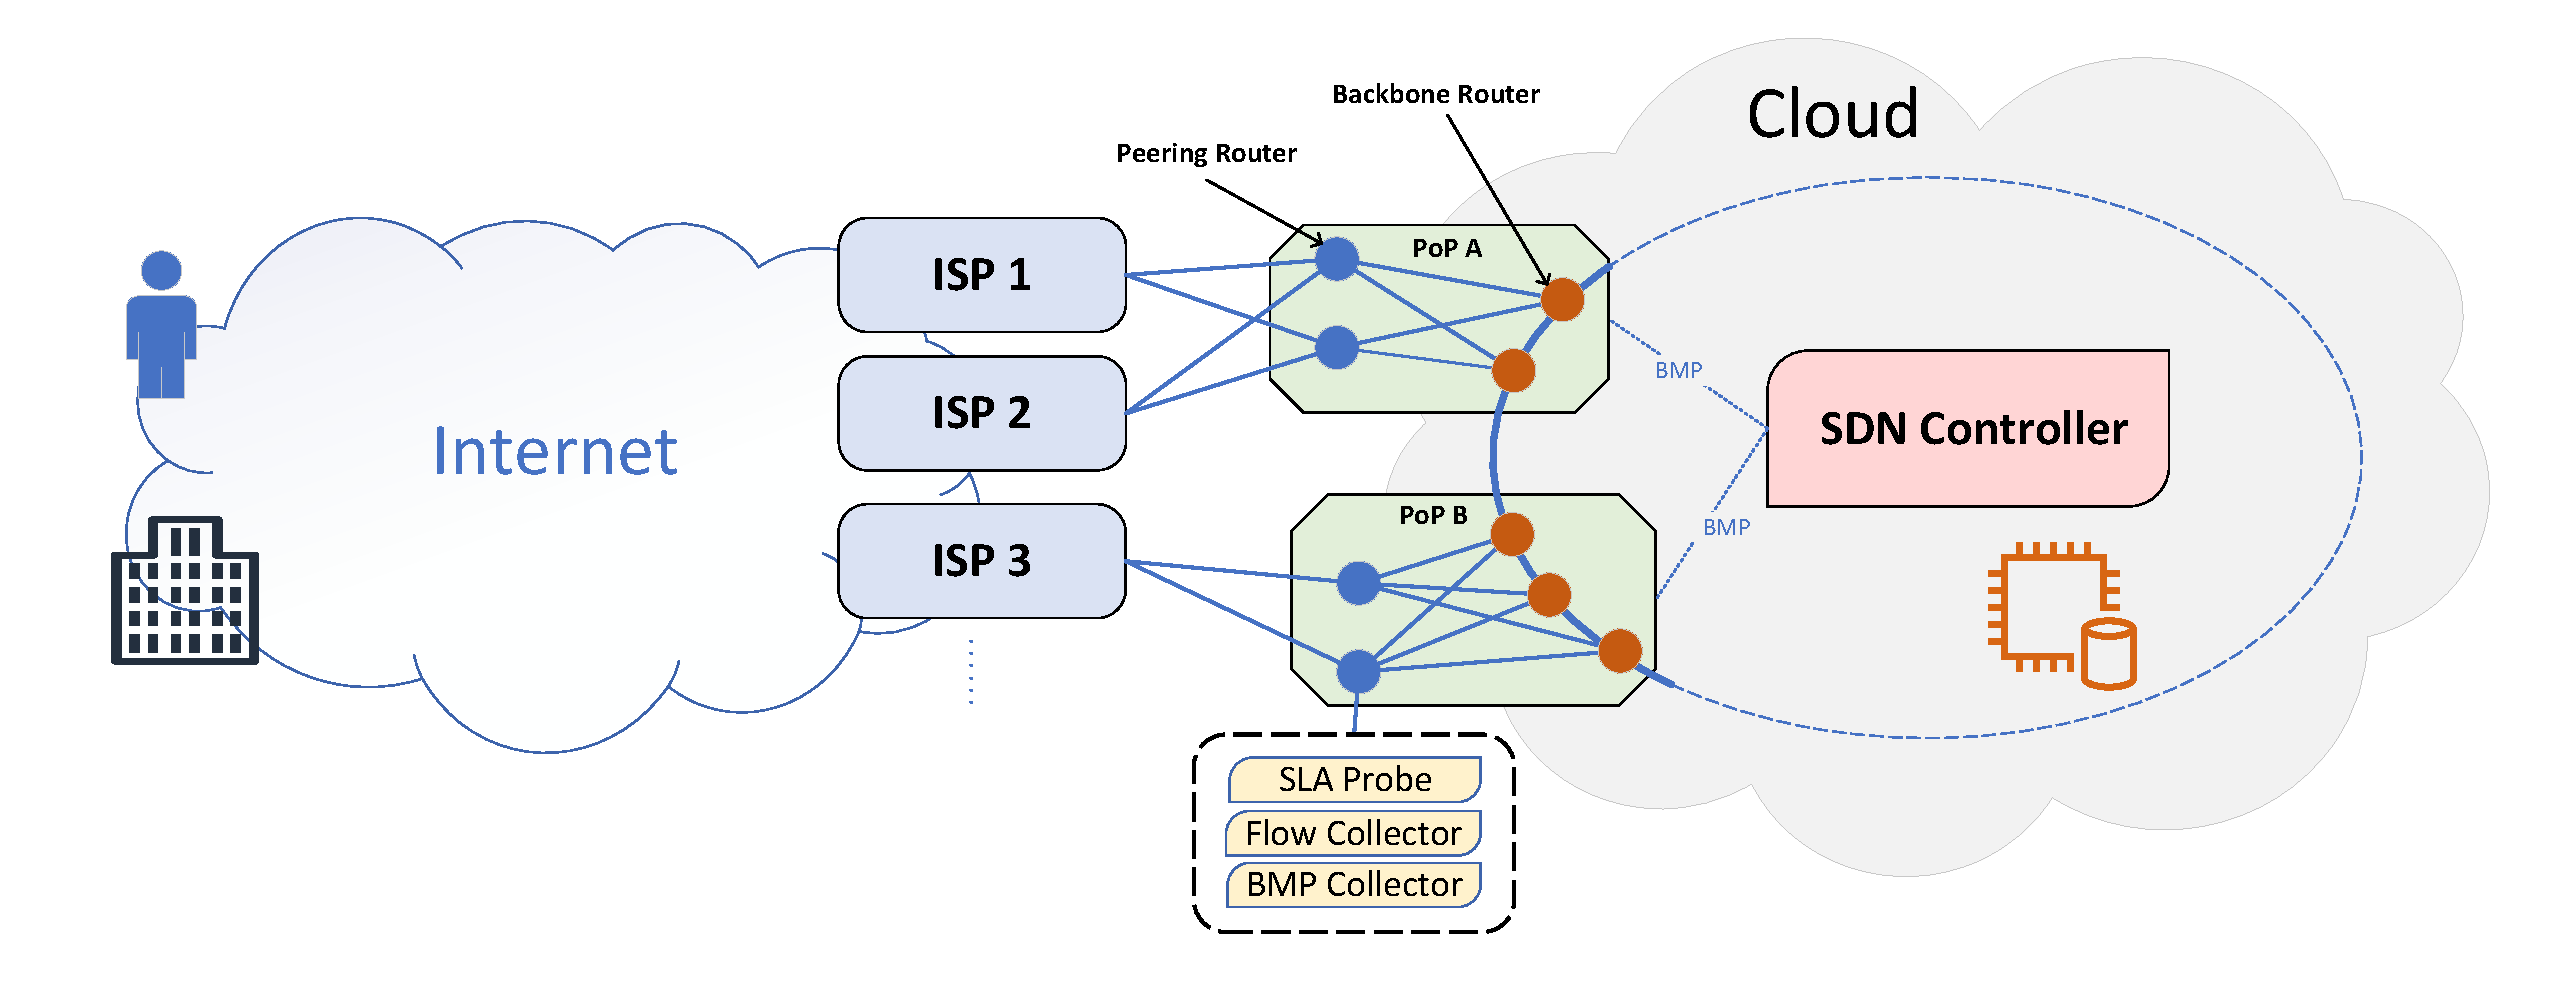
\includegraphics[width = 9cm]{figs/architecture/architecture.pdf}
	\caption{\small System architecture }
	\label{fig:systemar}
\end{figure}
\fi

\begin{figure}
	\centering
	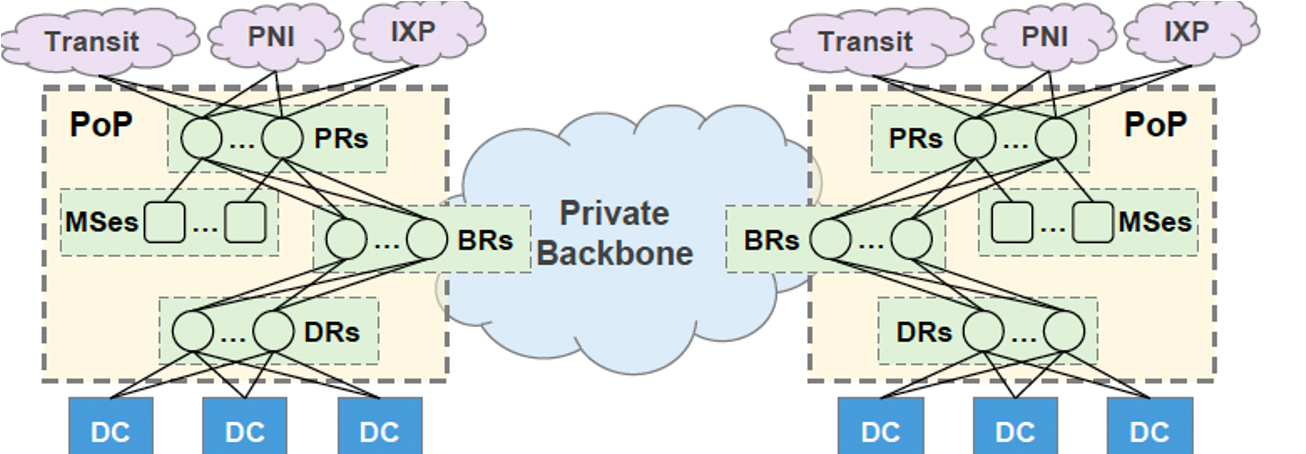
\includegraphics[width = 9cm]{figs/bg.png}
	\caption{\small Datacenters and PoPs are connected by a Private Backbone. Outbound traffic can then be routed to egress at any PoP.}
	\label{fig:bg}
\end{figure}

\subsection{Overview}  % {\sys} Architecture
We first briefly introduce the architecture of cloud network infrastructures. To serve cloud-scale geo-distributed users (as large as $O(10^{9})$ users), the cloud deployed multiple Point of Presences (PoPs) and data cetners globally. As shown in Figure \ref{fig:bg}, all PoPs are interconnected by a private backbone(private WAN) and multiple data centers are connected to PoPs. The outbound traffic from datacenter can go to any PoP in the same AS or any remote PoPs through private WAN. Each PoP hosts multiple Peering Routers (PRs) to connect with the Internet, backbone routers (BRs) to connect with the private backbone, and data center routers (DRs) to connect with datacenters. Each peering router is equipped with a monitoring server (MS) to monitor the link quality.

PRs in each PoP exchange BGP routes (a distinct set of public IP prefixes) with with transit providers, private network interconnects (PNIs), and Internet exchange points (IXPs) outside the PoP, which are associated with different Internet Service Providers (ISPs). Thus, traffic from or to these IP prefixes will be routed to the PoP by default. For the traditional routers, the routing is not aware of the traffic types. Google’s Espresso \cite{yap2017espresso}, Facebook EdgeFabric\cite{schlinker2017edgefabric}, and Tencent DSR \cite{shao21DSR} etc. To enable dynamic routings with fine-granularity traffics and enhance the capability of routes monitoring, we have built a hybrid architecture through commodity routers and programmable switches at PRs. 

% \para{Cloud edge.} Cloud edge contains BGP peers, {\egresses}, and PoPs. Cloud uses  {\egresses} $L$ between PoPs $V$ and BGP peers to connect to other ASes. At the edge of the cloud, each PoP comprises multiple routers, including peering routers that connect to BGP peers and backbone routers that interconnect with other backbone routers.

% \para{The WAN.} We formalize the Wide Area Network (WAN) $G$ as a directed graph, where the vertex set $V$ represents the PoPs and the edge set $E$ represents the backbone links between PoPs. Each edge $(u,v)\in E$ has capacity $C_{(u,v)}$, which is calculated by the original backbone capacity times 40\%, to spare some capacity to avoid congestion caused by demand spikes.

%\para{BGP peers.} BGP peers can be classified into several categories. Internet Protocol Transit (IPT) allows users to connect their networks to the public Internet. An Internet Exchange Point (IXP) is a physical facility that enables different networks to connect to each other directly. Private Network Interconnect (PNI) is a service that allows two or more private networks to connect to each other directly, making it convenient to share data or applications between their own networks without having to go through the public Internet. Only IPT provides routes to all prefixes worldwide because it has a default route. 

% \para{Peering contract.} There are three billing models \cite{singh2021costCascara} for inter-domain traffic prevalent on the Internet today: (1) Settlement-free (2) Per-port and (3) Per-Megabit. Settlement-free peers. Settlement-free peers agrees to exchange traffic with  each other at no cost (e.g., between cloud providers). In perport peering, a peer bills another for each network port used  at their facility (e.g., connections at IXPs). Per-Megabit is a utilization-based model where a network charges its peer based on the utilization of the link between them over monthly  billing cycles. % 需要补充的是95的复杂度 

% 介绍95的东西
Cloud providers sign contract with BGP peers for the  bandwidth usage to exchange traffic. The widely used billing model is based on the bandwidth utilization, i.e. the $95^{th}$ percentile billing model \cite{hong2013achieving}. Over the monthly billing cycle, bandwidth usage in peering link is recorded for every time slot (generally 5 minutes). 
The utilizations of megabits in every time slot are then sorted. The billing model charges the $95^{th}$ percentile of the utilizations. The top 5\% of usage over the billing period will not be counted. The $95^{th}$ percentile billing model has evolved as an industry standard on the Internet \cite{singh2021costCascara}. There can be a commit clause in this contract i.e., regardless of the actual usage, the customer commits to pay at least some pre-arranged amount to the provider. Specifically, in our network, IXPs do not charge based on usage, while IPT and PNI are charged based on $95^{th}$ percentile usage. The unit price of IPT is much higher than that of PNI. Conventionly, the cloud operators aim to minimize bandwidth cost on peering links billed by their utilization. However, the following two new trends lead to new challenge to the cloud network operators.


% The provider incurs costs to operate the network. Some Internet links are "private" or "owned," meaning that their cost only changes during capacity planning, which occurs a few times each year. The remaining egresses are charged based on usage. The bandwidth cost of these egresses is generally charged once a month, with pricing based on the 95th percentile usage being a common approach. 


\subsection{Peering Traffic Scheduling with regard to Backbone Constraints}
% problem and traditional solution
\para{Egress Scheduling}
Internet routing currently uses cost-driven policies to select one interdomain path per destination along which to direct traffic. To select one path amongst multiple policy-compliant ones, BGP uses particularly crude criteria rather than dynamically optimizing for performance. Notice that the bandwidth of the network inside each ISP is adequately provisioned, while the interconnecting bandwidth among the ISPs is relatively limited. Consequently, compare to the traffic inside one ISP, the traffic that crosses multiple ISPs usually suffers from higher latency and packet loss rate. Each ISP also serves as a transit provider, offering access to every publicly reachable destination IP address to our PoPs. In each PoP, each PR maintains BGP peer sessions with all of the three ISPs. When exchanging routes with our PRs, each ISP provides routes to all IP prefixes, and sets the preferred value of the routes to its hosted IP prefixes to a much higher value. As a result, for every IP prefix the route provided by its ISP will be selected as the BGP best path in our PRs. Therefore, traffic between each PoP and each IP address is inside one ISP by default, and thus achieves good performance without the constraint of limited inter-ISP bandwidth. 


\para{Internet TE considering the WAN's capacity.} Originally, traffic engineering for the Internet and the WAN has been operated independently. As a result, the Internet controller does not naturally introduce physical backbone links into the routing of Internet traffic, because the two functions have separate responsibilities and the WAN controller is transparent to the Internet controller. The WAN controller just provides a generalized estimate of the available inter-PoP capacity to the Internet controller. However, the traffic engineering approach significantly schedules large amounts of traffic between PoPs. We unfortunately discovered that the real capacity between some PoPs is severely limited. This discrepancy between the real capacity and the inaccurate available capacity rendered the schemes generated by the Internet controller ineffective. This experience has taught us that the joint management of Internet routing with backbone networks is much more important than we thought.


% It is essential to emphasize that {\sys} exclusively addresses Internet traffic and does not compute flow's actual path in the WAN. Instead, {\sys} does not compute the real path of flow $f$ in the WAN, but ensures that the scheme it generates adheres to WAN capacity constraints. And {\sys} also guarantees that the traffic allocation at each PoP in a given time slot aligns precisely with the scheme's specifications. 

\subsection{Differentiated Requirements for Network Services} 



\begin{table*}[tbp]
	\footnotesize
	\centering
	\begin{tabular}{c|c|c|c}
		\hline
		\bf{Service} & \bf{Scenario} & \bf{Demands} & \bf{ISP} \\
		\hline \hline
		Premium  & Game, Finance & Global performance-aware & \emph{All ISPs} \\
		\hline
		Latency-centric & Abroad Traffic & Specific Region performance-aware & International ISP \\
		\hline
	    Bandwidth-centric & IT business & Global Access, BW & Normal ISP \\
		\hline
	  Cost-centric & CDN, OBS & Low cost & IXP \\
		\hline
	\end{tabular}
        \vspace{-0.1in}
	\caption{\small Recommended choices of services in some scenarios}
	\label{table:classification}
\end{table*}

Customers have more and more strigent requirements on the path quality. Customers select the right network service based on their requirements and budget, which can change with the development. Take some customers in Table \ref{table:classification} as examples. For gaming and finance, rather than low price, users prefer Premium services to achieve latency as low as possible for speficied flows globally. Instead, for CDN and OBS services, users mainly focus on the low price of the path by choosing Cost-centric service. Therefore, we need the capability at data plane to identify the fine grain flows specified by users, and monitoring the paths quality for flow routes scheduling.


\iffalse
\begin{figure}
	\centering
	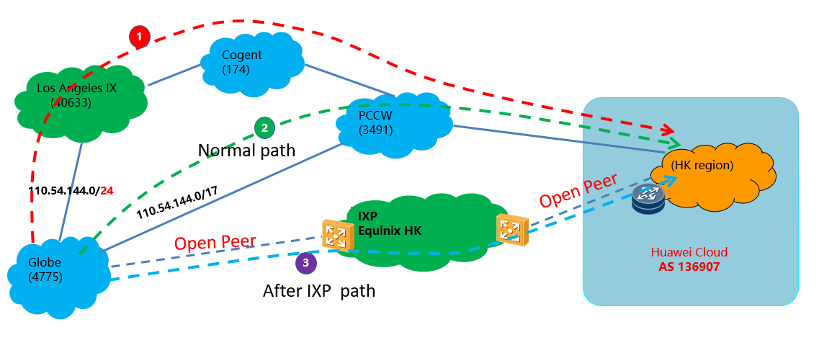
\includegraphics[width = 8cm]{figs/scheduling.png}
	\caption{\small Traffic scheduling through IDPR}
	\label{fig:design}
\end{figure}
\fi

\para{Monitoring} 
% 事前,多路径多出口探测,全覆盖规模大18K,ms-级时间戳
% DSCP标识, 流量复制,测量  % 聚类,top-k排序问题 
The data plane estimates loss and delay along different policy-compliant routes. It leverages programmable switches, i.e. the MS component as shown in Figure \ref{fig:bg},  are responsible for accurately and scalably measuring the delay of each egress port.
The monitoring subsystem uses an active IP collector to collect active IPs for each IP /24 prefix. The data about packet loss rate will be aggregated at AS-granularity. The volume of probing traffic is likely orders of magnitude less than the actual traffic, and some ISPs are known to treat probing traffic preferentially \cite{zhang2010optimizingEntact, valancius2013PECAN, liu2016Footprint}. More important, low-volume probing is inadequate for accurately measuring loss rate, while high-volume probing on all destinations via multiple paths would lead to significant extra load. {\sys} builds a simple mechanism to select representative IP addresses from active IP set: for each IP /24 block with more than ten active IP addresses, we randomly select ten of them as representative IP addresses; Otherwise, we select all of them as representative IP addresses The monitoring sub-system is out of the scope of this paper, please refer to our papers in ATC and SIGCOMM.\footnote{We remote the citations due to the requirement of ananymous!}. 

\subsection{Challenges}
By considering the joint management of Internet routing with backbones, as well as the fine grant performance-aware flows, we meet the following challenges. 

\begin{itemize}[leftmargin=*] 
\item \textit{Scheduling with multi-objective.} Practical and cost-efficient online edge TE. Since optimizing percentile costs is NP-Hard, finding optimal solutions can take several hours. We need an effective scheduling approach to solve the multi-objective problem which meet diverse demands of differerent suers while maintaining low operational cost.  
\item \textit{High computation complexity.} Given the fine grain traffic flows as well as the links associated with both peer routers and backbone, the optimization apporach grappled with the order of 1000x increase. 
\item \textit{Deployment for large volumn of flows.} We need a distrbuted control planes to realize the parallel computation. In additon, we need a more effective route compression approach in data planes to implement the routing deployment with regard to the scare memory (dozens of MB at best) in existing commodity switches.
\end{itemize}

To overcome these challenges, we introduce {\sys}, a cloud-scale public network scheduling system to meet the demand of performance-aware traffic management and satisfy the operational requirement, i.e. computation the $O(10^{10})$ routes within 10 seconds.

